\documentclass[a4paper,12pt]{extarticle}

% Даёшь нормальную кодировку!
\usepackage[utf8]{inputenc}

% Тщетные попытки включить Times New Roman
%\usepackage[T1]{fontenc}
%\usepackage{mathptmx}
%\usepackage{txfonts}

% Вставка картинок из директории images
\usepackage[dvips]{graphicx}
\graphicspath{{images/}}
\usepackage[usenames, dvipsnames]{color} % цвет

% Набор математических пакетов
\usepackage{amsmath}
\usepackage{amsfonts}
\usepackage{amssymb}
\usepackage{amsthm}
\usepackage{multirow}
\usepackage{tikz}

\usepackage{cmap} % поиск русских слов и вообще поддержка русского
\usepackage[english, russian]{babel}

\usepackage{listings}
\usepackage{verbatim}
\renewcommand{\lstlistingname}{Листинг}

\usepackage{statmodtitle}
\usepackage{indentfirst} % абзацный отступ после заголовка
\setcounter{tocdepth}{2} % Не отображать subsubsection и ниже в содержании
\bibliographystyle{unsrt}

% Поля и полуторный межстрочный интервал
\usepackage{setspace}
\usepackage[left=30mm,right=15mm,top=20mm,bottom=20mm]{geometry}
\onehalfspacing
% Начинать каждый раздел с новой страницы
\let\stdsection\section
\renewcommand\section{
    \newpage
    \stdsection
}

\setcounter{page}{2} % Резервируем первую страницу для титульного листа
\renewcommand{\arraystretch}{1.5} % Изменяем высоту строк таблицы

\lstset{ %
  backgroundcolor=\color{white},   % choose the background color; you must add \usepackage{color} or \usepackage{xcolor}
  basicstyle=\footnotesize,        % the size of the fonts that are used for the code
  breakatwhitespace=false,         % sets if automatic breaks should only happen at whitespace
  breaklines=true,                 % sets automatic line breaking
  captionpos=t,                    % sets the caption-position to bottom
  commentstyle=\color{green},    % comment style
  deletekeywords={...},            % if you want to delete keywords from the given language
  escapeinside={\%*}{*)},          % if you want to add LaTeX within your code
  extendedchars=true,              % lets you use non-ASCII characters; for 8-bits encodings only, does not work with UTF-8
%  frame=single,                    % adds a frame around the code
  keepspaces=true,                 % keeps spaces in text, useful for keeping indentation of code (possibly needs columns=flexible)
  keywordstyle=\color{blue},       % keyword style
  language=C++,                 % the language of the code
  morekeywords={*,...},            % if you want to add more keywords to the set
  numbers=left,                    % where to put the line-numbers; possible values are (none, left, right)
%  numbersep=5pt,                   % how far the line-numbers are from the code
%  numberstyle=\tiny\color{mygray}, % the style that is used for the line-numbers
  rulecolor=\color{black},         % if not set, the frame-color may be changed on line-breaks within not-black text (e.g. comments (green here))
  showspaces=false,                % show spaces everywhere adding particular underscores; it overrides 'showstringspaces'
  showstringspaces=false,          % underline spaces within strings only
  showtabs=false,                  % show tabs within strings adding particular underscores
  stepnumber=1,                    % the step between two line-numbers. If it's 1, each line will be numbered
  stringstyle=\color{mymauve},     % string literal style
  tabsize=4,                       % sets default tabsize to 2 spaces
  title=\lstname,                   % show the filename of files included with \lstinputlisting; also try caption instead of title
  basicstyle=\footnotesize\ttfamily,
  keywordstyle=\bfseries\color{green!40!black},
  commentstyle=\itshape\color{purple!40!black},
  identifierstyle=\color{blue},
  stringstyle=\color{orange}
}

% всё тлен и безысходность

\date{2012-06-19}
\title{Разработка интерактивной системы визуализации данных в физических моделях}
\author{Зайцев Вадим, ФИТ НГУ, 9204}

\begin{document}

\tableofcontents

\section*{Введение}
\addcontentsline{toc}{section}{Введение} % Добавляем в содержание раздел без номера
\label{sec:intro}

Тут должен быть краткий обзор предметной области (о моделировании (краткая классификация), мы выбираем имитационное моделирование, мелкозернистый параллелизм, его использования для моделирования)
Цель, актуальность, план следующего изложения.

Необходимость постановки опыта (или эксперимента) над системой (под системой понимается совокупность объектов, функционирующих и взаимодействуюищих друг с другом для достижения определённой цели – в [2] написано, что такое определение даётся в [Шмидт, Тэйлор, 1970]) возникает постоянно и в самых различных в сферах деятельности, будь то физические процессы, экономические системы и т.д. Однако, во-первых, произвести эксперимент над реальной системой не всегда представляется возможным в силу того, что системы может либо не существовать, либо в результате эксперимента будет невозможным её возвращение в исходное состояние, а, во-вторых, эксперимент над реально существующей системой может потребовать слишком больших затрат на его осуществление. В таких случаях возможно прибегнуть к моделированию: построить модель – упрощённый вариант системы (что-нить о том, что этот вариант должен обладать требуемым свойствами) – и провести эксперимент уже над моделью. На этапе построения модели необходимо сделать выбор между физической моделью (создание упрощённого, но реального существующего варианта системы для проведение эксперимента) и математической (описание системы посредством отношений, которые определяют как система будет реагировать на изменения, если бы она существовала). Математическая модель может иметь точное аналитическое решение, дающее представление о том, как входные параметры влияют на систему в соответствие с построенной моделью. Однако описываемые модель отношения могут не дать простого аналитического решения и потребовать огромных вычислительных ресурсов, что сделает невозможным аналитическое моделирование или потребует большего упрощения системы. Альтернативный вариант в таком случае: изучение системы с помощью имитационного моделирования, то есть многократного испытания модели с нужными входными данным. Имитационные модели за последнее время получили широкое распространение благодаря появлению инструментов, упрощающих создание компьютерных программ, и увеличению и удешвлению компьютерных мощностей.  [2, стр. 23-34]
сказать, что моделирование может быть физическим, аналитическим, но мы будем рассматривать имитационное
Однако, моделирование невозможно без инструмента визуализации, позволяющего изучать модель и исследовать результаты смоделированного эксперимента: работа с объектами на данных микроуровне чрезвычайно сложна, т. к. он представляет из себя огромный массив ячеек с частицами, в то время как визуализация позволяет получить качественную картину ???. Целью данной работы является разработка подсистемы пользовательского интерфейса и визуализации данных среды имитационного моделирования, назначение которой – построение и исследование клеточно-автоматных моделей, широко применяющихся для исследования явлений естественных наук. К системе предъявляются требования, 

Цель работы — обеспечить исследователя \textit{МЗП} моделей физических процессов инструментом для построения и отладки таких моделей и визуализации данных в них. Хотя система должна обладать достаточной универсальностью и быть пригодной для широкого спектра таких моделей, в первую очередь рассматривается визуализация данных для клеточно-автоматных моделей газов. 
Актуальность. Рассматриваемый класс моделей характерен сложностью происходящих в них преобразований данных и большим объемом данных. Под большим объемом данных подразумевается, что он существенно превосходит размеры основной памяти. Сложность преобразований данных в моделях означает необходимость: 1) отладки модели в процессе ее создания и 2) создания режимов отображения, позволяющих исследователю увидеть как точную количественную картину некоторого фрагмента состояния модели, так и качественную картину протекающих в модели процессов. Если исследователь выбирает путь построения собственной программы визуализации, он неизбежно сталкивается с необходимостью реализации системных функций, сложность которых значительно выше, чем само описание модели.  Таком образом, для эффективной работы исследователя необходим инструмент для построения, отладки и исследования моделей.







Далее в работе будет описан процесс разработки системы по этапам. В первую очередь были предъявлены требования к разрабатываемой системе, главными из которых являются: адекватность предметной области и открытость, в разделе «2 Формирование требований» будет подробно раскрыто каждое из требований, обусловлено наличие их предъявление к создаваемой системе. В разделе «3 Обзор существующих систем» представлен краткий обзор уже имеющихся систем визуализации в исследуемой предметной области, исследование их на соответсвие сформулированным ранее требованиям, сравнение по требуемым параметрам. В разделе «4 ???» разобрана архитектура разработанной системы, детально описан каждый компонент системы: тутнуженглагол цель создания данного модуля системы, какие из поставленных задач он решает и каким требованиями удовлетворяет, список основных функций, которые он реализовывает. Надо ли писать про заключение?




\section{Формирование требований}
\label{sec:requirements}

Назначение системы --- визуализация данных в МЗП моделях физических процессов.  Наиболее существенное требование, требование адекватности системы проблемной области, заключается в создании удобного инструмента, содержащего все необходимые исследователю функции для изучения широкого спектра таких моделей.

Моделирования физических явлений с помощью моделей с мелкозернистым параллелизмом --- динамично развивающаяся область, в которой постоянно возникают новые классы моделей. Для того, чтобы система могла применяться для них, она должна иметь открытую архитектуру, позволяя пополнять свой набор функций не только разработчикам, но и пользователям системы. 

Для МЗП моделей физических явлений характерно то, что адекватность резульатов достигается только при очень больших размерах объектов: во-первых, не все являения могут быть заметны на моделях маленького размера, во-вторых, за счёт увеличения размера объекта достигается более точный результат.

Таким образом, основными требованиями, предъявляемыми к системе, являются:
\begin{itemize}
    \item адекватность проблемной области;
    \item открытая архитектуа;
    \item обработка больших объёмов данных;
\end{itemize}

Рассмотрим более подробно, что включает в себя каждое из приведённых требований.

\begin{subsection}{Адекватность проблемной области}
    \label{sec:requirements-adequacy}

    Адекватность системы предметной области означает удовлетворение системой требованиям, которые предъявляет к ней исследователь в данной предметной области: так как система создаётся для работы с клеточно-автоматными моделями, то она должна реализовывать необходимые функции, требующиеся при изучении данной обалсти, а именно:
    \begin{itemize}
        \item построение моделей;
        \item управление проектами;
        \item исполнение модели;
        \item изучение модели;
        \item отладка модели.
    \end{itemize}

    \begin{subsubsection}{Построение моделей}
        С точки зрения системы модель представляет из себя непосредственно свойства модели как физического объекта (т. е. все свойства модели: например, для моделей клеточных автоматов это будут правила, по которым которым осуществляются переходы в ячейках, массы частиц покоя и количество движущихся частиц) и объекты данных, над которым производятся вычисления. Объектом данных является структура, хранящая в себе состояние моделируемого объекта. Такая структура может быть как и многомерный массив так и нерегулярная структура данных.
        
        Исследователю необходимо иметь возможность формировать и корректировать параметры модели и создавать и редактировать объекты данных. Для работы с моделью удобно наличие визуальной среды: графический пользовательский интерфейс упрощает работу с множеством параметров модели и с большими объектами данных.
        
        Свойства модели могут быть значениями произвольного содержания (число, строка, массив значений и т. п.). Объект данных может быть как небольшого (обычно такие объекты используются при отладке модели), так и огромного размера. И в том, и в другом случае бывает необходимость редактировать и значения отдельных ячеек, и сразу большой области объекта данных.
    \end{subsubsection}
        
    \begin{subsubsection}{Управление проектами}
        В процессе исследования возникает необходимость скорректировать параметры изучаемой модели, посмотреть на изменение поведения, сравнить данную модель с исходной по каким-либо характеристикам. В таких случаях удобно объединять две и более модели в один проект с возможностью сохранения и загрузки проекта. 
        
        Проект можно определить как группу логически связанных между собой моделей, при этом определение модели расширяется, в проекте с моделью так же ассоциируются пользовательские настройки (например, сохранение настроек режимов отображения для данной модели). пользовательские настройки, набор операций. В проект можно добавлять новые модели, удалять из него старые. Должна быть поддержка сохранения открытого проекта с возможностью последующей загрузки.
    \end{subsubsection}
        
    \begin{subsubsection}{Исполнение модели} 
        Одной из основных функций является счёт модели: это включает в себя передачу параметров модели и объекта данных на вычислитель, запуск модели на фиксированное число итераций, ожидание завершения счёта и последующее получение результирующих данных с вычислителя.
        
        Под вычислителем понимается устройство, на котором происходит моделирование. Вычислителем может выступать такое устройство локального или удалённого компьютера, как центральный или графический процессор. Вычислитель при этом необязательно является однопроцессерной машиной: в его роли могут так же выступать мультипроцессорные системы, системы с распределённой памятью, кластеры и ГРИД-системы.
    \end{subsubsection}
        
    \begin{subsubsection}{Изучение модели}
        При работе с моделями пользователь системы нуждается в  работате с объектом данных модели не только на микроуровне, но и с качественной картиной: иметь возможность выделить из всего объекта данных какую-либо конкретную характеристику. Так же пользователю необходимо дать возможность взаимодействовать с системой, быть не только наблюдетелем за процессом моделирования, но и иметь средства как-то влиять на него, т. е. обеспечить интерактивность.
        
        Качественная картина может быть предоставлена за счёт поддержки различных режимов отображения (режимом отображения является функция, отображающая объект данных в изображение, которое впоследствии может быть выведено на экран монитора): например, это может быть режим осреднённых плотностей или профиль волны для исследования её поведения. Полезными могут быть не только режимы, визуализирующие какую-либо конкретную характеристику (плотность частиц, направление потоков), но и режимы, формирующие целостную картину: например, трёхмерный режим с возможностью масштабирования и вращения для просмотра объекта данных с разных ракурсов.
    \end{subsubsection}
        
    \begin{subsubsection}{Отладка модели}
        При построении бoльших и сложных моделей могут возникать ошибки в их описании. В таких случаях модель приходится отлаживать: использовать какие-либо средства с целью выявления допущенных ошибок. Система в свою очередь должна помочь исследователю, предоставив такие средства.
        
        В процессе отладки востребован не только запуск счёта модели на фиксированное, большое количество итераций, но и запуск модели в режиме пошагового исполнения: формирование модели и отправка её на вычислитель, запуск на небольшое количество шагов, получение результирующих данных с возможностью продолжить вычисления с того момента, где они были приостановлены. Пошаговое исполнение позволяет детальнее изучить поведение модели.
        
        Так же при отладке востребованной может оказаться возможность модификации текущего объекта данных, передача изменений на вычислитель и продолжение счёта.
    \end{subsubsection}

\end{subsection}

\begin{subsection}{Открытая архитектура}
    \label{sec:requirements-open}
    
    Открытость архитектуры облегчает сопровождение системы и её адаптация к изменяющимся требованиям.

    Свойство открытости включает в себя:
    \begin{itemize}
        \item расширяемость;
        \item переносимость;
        \item интероперабельность;
        \item дружественность пользовательского интерфейса.
    \end{itemize}

    \begin{subsubsection}{Расширяемость}
        \textit{Пользователи уже используют свои форматы, они от них не уйдут, мы сами не может предоставить поддержку всего-всего, потому предоставляем средства для вклчения поддержки} Система должна быть готова к изменениям, связанным с включением поддержки новых классов моделей, ранее не предусмотренных системой. Это обусловлено тем, что требуется создание универсального инструмента, реализующего не только необходимый на данный момент функционал, но и способного в будущем адаптироваться под новые требования, предоставляющего механизм для встраивания нового функционала.
        
        Направлениями для расширения системы являются:
        \begin{itemize}
            \item режимы отображения;
            \item поддержка графических библиотек;
            \item коммуникация с подсистемой моделирования.
        \end{itemize}
        
        \textit{расписать направление расширяемости по пунктам} Помимо поддержки новых форматов данных и новых классов моделей, так же должна быть возможность встраивать поддержку новых графических библиотек (например, отрисовку трёхмерных изображений на ОС Windows делать не с помощью OpenGL, а с использованием библиотеки Direct3D). Другим направлением расширением системы может быть добавление поддрежки альтернативных способов коммуникации с вычислителем: например, когда в качестве вычислителя вместо центрального процессора выступает видеокарта, то обмен данными уже невозможно организовать через общую память и потребуется реализовать передачу данных между оперативной памятью компьютера (к которой система визуализации имеет прямой доступ) и памятью графического ускорителя.
        
        Всё это требует от системы масштабируемости по архитектуре: возможность вносить изменения, связанные с добавлением нового функционала, при этом минимизируя влияние (т.е. либо не требуя модификации, либо модификация существующей реализации должна быть незначительной) на другие, уже существующие компоненты системы.
    \end{subsubsection}
        
    \begin{subsubsection}{Переносимость}
        С течением времени архитектуры процессоров и операционные системы меняются. Создание системы, привязанной к одной конкретной платформе, может в будущем потребовать значительных усилий для портирования системы под другую платформу или вовсе привести к прекращению поддержки системы, когда используемая платформа устареет.
        
        Второй проблемой при разработке платформозависимой системы является проблема взаимодействия с приложениями, привязанными к другим платформам. Это потребует от пользователей либо портировать их приложения на используемую системой платформу, либо отказаться от использования системы.
        
        Таким образом, от системы требуется свойство переносимости --- отсутствие  зависимостей модулей системы от конкретной платформы. В системе допускается привязка отдельных реализаций некоторых компонентов к определённым платформам, но в целом она должна оставаться платформонезависимой.
        
        Переносимость должна быть обеспечена на уровне исходного кода (код прилоежния не должен использовать платформозависимые библиотеки или функции или же функциональность, достигаемая с использованием данных библиотек, должна быть реализована для каждой платформы) и на уровне данных (работа с созданными проектами и моделями на одной платофрме должна быть возможна и на других платформах) [3, page 27].
    \end{subsubsection}
        
    \begin{subsubsection}{Интероперабельность}
        Свойство интероперабельности означает способность системы взаимодействовать с окружением, в котором она запущена. Для подсистемы визуализации это, в первую очередь, способоность взаимодействовать с подсистемой моделирования.
        
        Взаимодействие основывается на использовании общих форматов хранения данных, интерфейсов для взаимодействия на локальных системах или пртоколв для взаимодействия в распределённых средах. Благодаря интероперабельности система визуализации может использоваться как звено в цепи обработки информации, поулчая входыне данные от подсистемы моделирования, отрисовывая полученные данные и передвавая полученные изображения другим приложениям для последующей обработки.
    \end{subsubsection}
        
    \begin{subsubsection}{Дружественность интерфейса}
        Интерфейс системы можно разделить на интерфейс пользователя и программный интерфейс.
        
        Дружественность пользовательского интерфейса заключается в наличии интуитивно-понятного и комфортного взаимодействия системы с пользователем. Требование является необходиым для любой отчуждаемой от разработчиков программы, в которой присутствует функция взимодействия с пользователем.
        
        Дружественность программного интерфейса относится к разработчикам системы (как и к тем, кто изначально разрабывает систему, так и к пользователям, которые будут расширять систему за счёт встраивания своих модулей) и означает упрощение разработки системы: интерфейсы, дающие возможности для расширения системы, должны требовать реализацию только минимального необходимого набора методов.
    \end{subsubsection}

\end{subsection}

\subsection{Обработка больших объёмов данных}

Требование к поддержки больших объёмов данных обусловлено особенностью моделей физических являений:
\begin{enumerate}
    \item Многие явление могут быть незаметны на моделях маленького размера (например, вихри --- они проявляются только на объектах больших размеров).
    
    \item Как правило, при увеличиении размера объекта данных, при более сильном дроблении, качество моделирования повышается и результат получается более точным.
\end{enumerate}

Под возможностью обработки больших объёмов данных понимается способность системы визуализировать объекты данных, размер которых превышают размер оперативной памяти компьютера.


\begin{section}{Обзор существующих систем}

Имитационное моделирование, а значит и необходимость в средствах визуализации, существует уже достаточно давно, потому следующим этапом после формирования требований был обзор уже существующих систем.

Далее приведён обзор нескольких, \textit{уточнить каких}, систем. Полный список обозреваемых систем и их соответствие требованиям привдён в Приложении А. 

\begin{subsection}{Mirek's Celebration}
    Система моделирования 1D и 2D клеточно-автоматных моделей.
    Имееет удобный, интуитивно понятный пользовательский интерфейс, хорошо документирована.

    \begin{table}[h]
        \caption{Соответствие требованиям системы Mirek's Celebration}
        \label{tabular:mirekscell}
        \begin{center}
            \begin{tabular}{|p{0.35\linewidth}|p{0.05\linewidth}|p{0.5\linewidth}|} \hline
                Адекватность пред. области & + & \\ \hline
                Расширяемость              & $\mp$ & Есть возможности встраивания DLL. Возможности расширения всё-таки ограничены. \\ \hline
                Интероперабельность        & ?? & \\ \hline
                Платформонезависимость     & -- & Win32 \\ \hline
                Дружественный интерфейс    & + & \\ \hline
                Большие объёмы данных      & -- & \\ \hline
            \end{tabular}
        \end{center}
    \end{table}
\end{subsection}

\begin{subsection}{WinALT}
    Система моделирования разнообразных клеточно-автоматных моделей.

    \begin{table}[h]
        \caption{Соответствие требованиям системы WinALT}
        \label{tabular:winalt}
        \begin{center}
            \begin{tabular}{|p{0.35\linewidth}|p{0.05\linewidth}|p{0.5\linewidth}|} \hline
                Адекватность пред. области & -- & Система рассчитана на проектирование МЗП алгоритмов и структур. \\ \hline
                Расширяемость              & + & \\ \hline
                Интероперабельность        & + & \\ \hline
                Платформонезависимость     & ?? & Win32 \\ \hline
                Дружественный интерфейс    & + & \\ \hline
                Большие объёмы данных      & -- & \\ \hline
            \end{tabular}
        \end{center}
    \end{table}
\end{subsection}

\begin{subsection}{Ansys Fluent}
    Система моделирования широкого спектра физических процессов, в том числе и газовой динамики, обладает богатыми возможностями моделирования и визуализации.

    \begin{table}[h]
        \caption{Соответствие требованиям системы Ansys Fluent}
        \label{tabular:ansysfluent}
        \begin{center}
            \begin{tabular}{|p{0.35\linewidth}|p{0.05\linewidth}|p{0.5\linewidth}|} \hline
                Адекватность пред. области & -- & Дифференциальные уравнения решаются классическими методами. \\ \hline
                Расширяемость              & + & Возможность встраивания пользовательских функций. \\ \hline
                Интероперабельность        & + & \\ \hline
                Платформонезависимость     & ?? & \\ \hline
                Дружественный интерфейс    & + & \\ \hline
                Большие объёмы данных      & ?? & \\ \hline
            \end{tabular}
        \end{center}
    \end{table}
\end{subsection}

\subsection{Выводы}

Таким образом, ни одна из рассмотренных систем в полной мере не удовлетворяет всем предъявленным к ней требованиям и было решено создать собственную реализацию системы визуализации. На рисунке~\ref{systems-simulus} графически изображено \textit{...}

\begin{figure}[h]
    \center{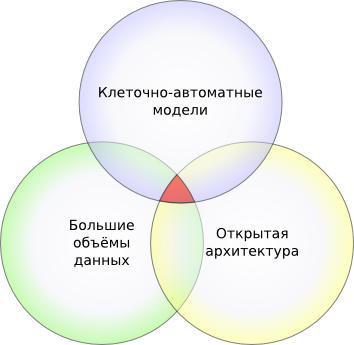
\includegraphics[width=.5\linewidth]{systems-simulus}}
    \caption{Существующие системы визуализации}
    \label{ris:systems-simulus}
\end{figure}

\end{section}



\section{Архитектура системы}
\label{sec:architecture}

На верхнем уровне архитектура системы представляет из себя 4 взаимодействующих друг с другом модуля:
\begin{itemize}
    \item модуль взаимодействия с подсистемой моделирования;
    \item модуль поддержки графических библиотек;
    \item модуль поддержки различных режимов отображения;
    \item пользователский интерфейс.
\end{itemize}
\textit{Структура системы такова (см. рис??)...} Графически/Схематически модульная архитектура системы представлена на Рис.~\ref{ris:architecture-all}. 
\textit{Так же рисунок, на котором изображены зависимости между модулями}.

\textit{Модульное программирование. ООП.}

\begin{figure}[h]
    \center{\includegraphics[width=1\linewidth]{architecture}}
    \caption{Архитектура подсистемы визуализации}
    \label{ris:architecture-all}
\end{figure}

Такая модульная/отркытая архитектура системы, разбивающая систему на отдельные, взимодействиующие между собой части, реализаций которых одна от другой никак не зависят, позволяет вносить изменения (как модификация существующей реализации, так и расширение за счёт \textit{чего-то нового}) в отдельные компонеты прозрачно для остальных.

\begin{subsection}{Модуль взаимодействия с подсистемой моделирования}
    \label{sec:architecture-calc}
    \begin{figure}[h]
        \center{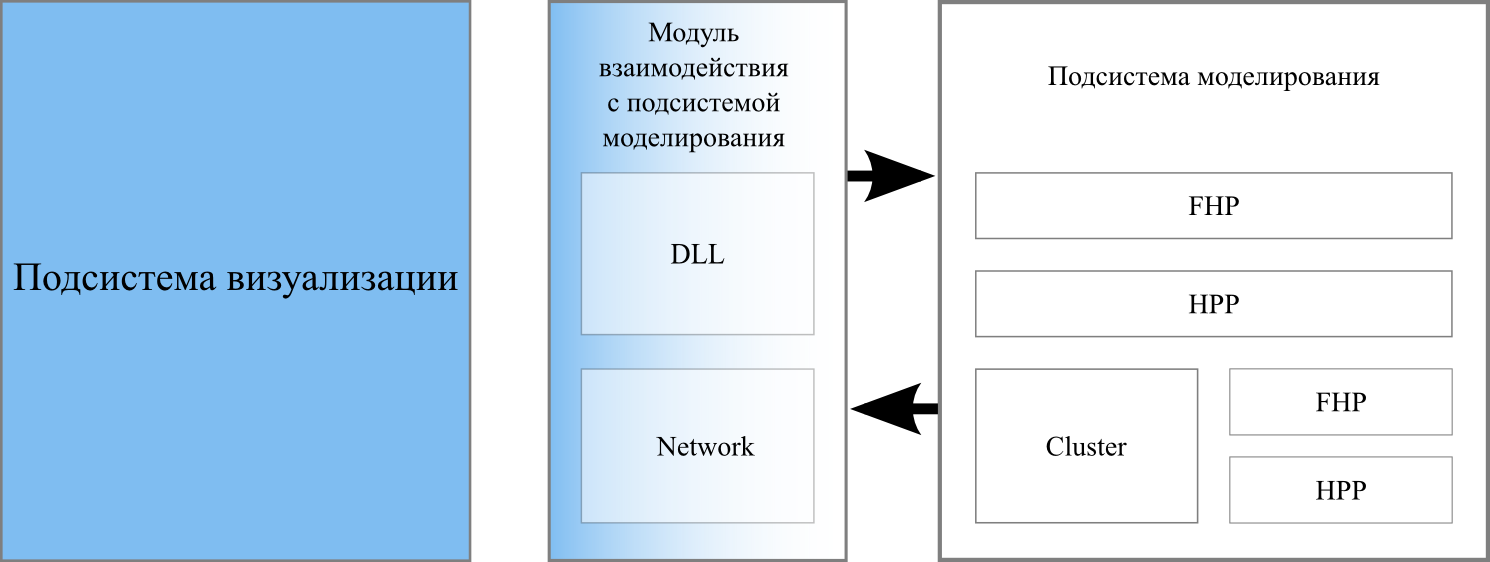
\includegraphics[width=1\linewidth]{architecture-calc}}
        \caption{Модуль взаимодействия с подсистемой моделирования}
        \label{ris:architecture-calc}
    \end{figure}
    
    Для обеспечения коммуникации подсистемы визуализации с подсистемой моделирования был создан интерфейс для подключения вычислителей.

    В основные функции, решаемые данным модулем, входит запуск процесса моделирования в синхронном (запуск на счёт фиксированного количества итераций, ожидание завершения моделирования и получение результата) и в асинхронном (запуск на счёт с возможностью подключения к вычислителю в любой момент и получения текущего состояния \textit{чего???}) режимах и реализация протокола передачи объекта данных визуализатору с вычислителя.

    Класс возможных вычислителей, с которыми может коммуницировать подсистема визуализации, программно ничем не ограничен. Таким образом, в качестве вычислителя может выступать \textit{абсолютно любое устройство}: как процессор или видеокарта локальной машины, так и удалённый кластер, который, возможно, требует подключения по специфичному??? протоколу (вполне стандартна ситуация, когда доступ к кластеру осуществляется по SSH с необходимость авторизации).

    Подключение нового вычислителя осуществляется написанием реализации созданного интерфейса.
    \textit{Может, ссылку на приложение, которое создать для каждого модуля, где будет кратко описано, как создавать реализацию нового модуля?}. На данный момент реализована поддержка разделяемых библиотек для запуска счёта на локальной машине и в процессе разработки поддержка запуска счёта на удалённой машине, в том числе и для моделирования на кластере.

    Т.о. система удовлетворяет свойству интероперабельности. <- \textit{надо куда-то красивее вписать}.
\end{subsection}

\begin{subsection}{Модуль поддержки графических библиотек}
    \label{sec:architecture-graphics}
    \begin{figure}[h]
        \center{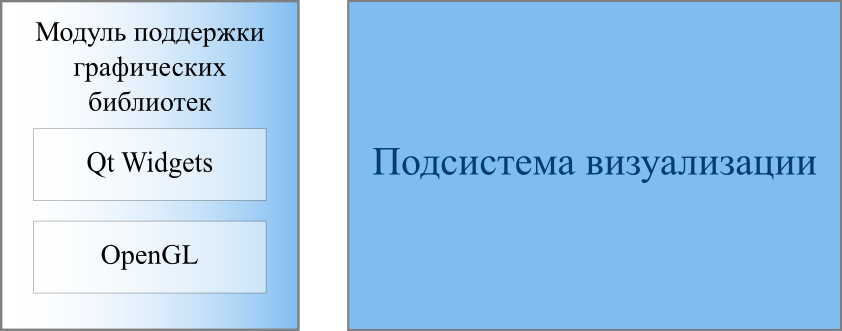
\includegraphics[width=.6\linewidth]{architecture-graphics}}
        \caption{Модуль поддержки графических библиотек}
        \label{ris:architecture-graphics}
    \end{figure}
    
    Посколько основной задачей инструмента визуализации является \textit{отрисовка} изображения, то в состав системы так же был включён модуль, отвечающий за поддержку различных графических библиотек. На данный момент существует множество библиотек, как для работы с двухмерной графикой (GTK, Qt, wxWidgets и многие другие) и с трёхмерной графикой (OpenGL, Direct3D и т.д.) и основной задачей модуля является предоставление общего интерфейса для рисования независимо от того, какая из библиотек используется в данный момент для формирования итогового изображения.

    Модуль поддрежки графических библиотек, как и модуль взаимодействия с подсистемой моделирования, представлет из себя интерфейс, реализацией которого осуществляет подключения новых библиотек. В интерфейс входит рисование графических 2D и 3D примитивов (точки, линии, закрашивание областей), рисование более сложных объектов (различного рода кривые, объединение и пересечение объектов), поддержка прозрачности, если таковая есть в библиотеки. Иными словами, задачей интерфейса является предоставление \textit{универсального} доступа к возможностям библиотек, скрыв при этом различия при работе с ними для других модулей. \textit{Сказать про возможноую зависимость библиотек и платформ?}.

    За счёт введения интерфейса достигается расширяемость, а отсутствие привязанности интерфейса к каким-либо конкретным технологиям делает систему переносимой. Стоит отметить, что некоторые графические библиотеки являются платформозависимыми (например, возожность использовать Direct3D имеется только под операционной системой Microsoft Windows), однако, в целом это не делает систему непереносимой.

    На данный момент используются следующие кроссплатформенные библиотеки:
    \begin{itemize}
        \item Модули QtGUI и QtWidgets из библиотеки Qt.
        \item Библиотека OpenGL для отрисовки 3D изображений.
    \end{itemize}
    \textit{Как подключить новые библиотеки?}
\end{subsection}

\begin{subsection}{Модуль поддержки режимов отображения}
    \label{sec:architecture-render}
    \begin{figure}[h]
        \center{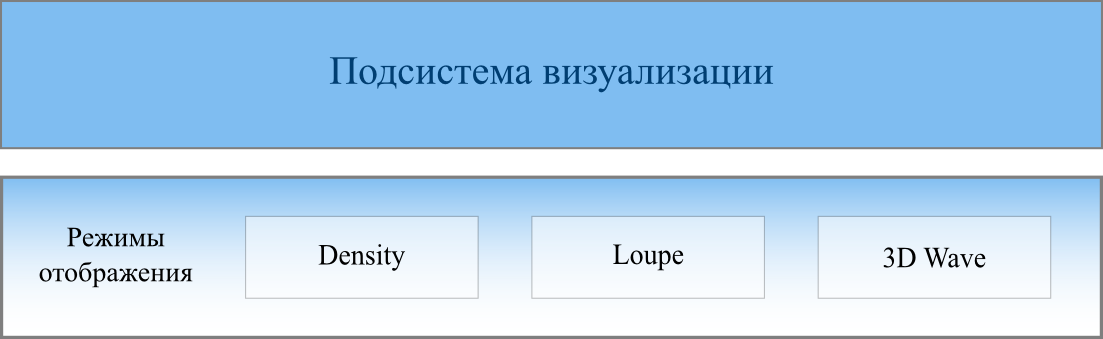
\includegraphics[width=.8\linewidth]{architecture-render}}
        \caption{Модуль поддержки графических библиотек}
        \label{ris:architecture-render}
    \end{figure}
    
    В разделе \ref{sec:requirements-adequacy} одним из требований, предъявлемых к системе, является предоставление исследователю как возможность наблюдать за изменениями отдельных различных характеристик, так и возможность увидеть целостную картину. Данный модуль реализует поддержку различных режимов отобржения и предоставляет возможности для встраивания новых режимов.

    Единственная функция, которую реализует модуль поддержки режимов отображения, это отображение части или всего объекта данных в двухмерное или трёхмерное изображение. При отрисовывании изображения данный модуль использует интерфейс, предоставляемый модулем поддержки графических библиотек, а работа с объектом данных модели происходит через модуль взаимодействия с подсистемой моделирования. 

    С помощью данного модуля достигается расширяемость системы: появляется возможность встраивать новые режимы отображения, при этом не затрагивая обмен данных с вычислительной подсистемой и не внося изменения в существующие форматы данных.

    Реализации поддержки режима отображения включает в себя реализацию двух \textit{компонентов}: функцию
    Написать про возможность выделение слоёв (переиспользуемые компоненты), сборку из слоёв.
    Для поддержки различных режимов отображения был так же разработан интерфейс для их подключения, что делает систему расширяемой. На данный момент релизованы:
    \begin{itemize}
        \item Режим осреднения (статистически-обобщённый).
        \item Режим лупы, позволяющий рабоатть с объектами данных на микроуровне.
        \item 3D режим для получения полноценной картины.
    \end{itemize}
\end{subsection}

\begin{subsection}{Модуль пользовательского интерфейса}
    \label{sec:architecture-ui}
    Для взаимодействия с пользователем системы был реализован графический интерфейс. Задачей модуля было предоставить пользователю простой, но в тоже время функиональный, удобный, интуитивно-понятный интерфейс. Графический интерфейс направлен на удовлетворение свойству адекватности предметной области: через него пользователь осуществляет работу с проектами и моделями, запуск и наблюдение за процессом моделирования, получение и исследование результатов моделирования, наличие средств для отладки модели.
    
    \textit{Представляет из себя MDI интерфейс. Подбробнее --- в приложении.}
\end{subsection}


\section*{Заключение}
\addcontentsline{toc}{section}{Заключение} % Добавляем в содержание раздел без номера

В результате работы была разработана архитектура подсистемы визуализации системы имитационного моделирования, на основе разработанной архитектуры была написана реализация системы. Был разработан и опробован на чём? механизм взаимодействия с моделью. Разработан механизм встраивания режимов визуализации, на базе которого построено несколько режимов каких? Разработана графическая оболочка системы.
В планах реализация механизма удалённого исполнения модельных программ, запуск счёта модели на кластере ССКЦ.

\section*{Приложение А. Сравнение систем визуализации}
\begin{center}
    (Обязательное)
\end{center}
\addcontentsline{toc}{section}{Приложение А. Сравнение систем визуализации}

\begin{table}[h]
        \caption{Соответствие систем визулизации предъявленным требованиям}
        \label{tabular:ansysfluent}
        \begin{center}
            \begin{tabular}{|p{0.4\linewidth}|c|c|} \hline
                \textbf{Система}    & \textbf{А} & \textbf{Р} \\ \hline
                Mirek's Celebration & +          & $\mp$      \\ \hline
                WinALT              & +          & +          \\ \hline
            \end{tabular}
        \end{center}
    \end{table}

\section*{Приложение Б. Реализация модуля взимодействия с подсистемой моделирования}
\begin{center}
    (Рекомендуемое)
\end{center}
\renewcommand{\thesubsection}{\Asbuk{section}.\arabic{subsection}}
\setcounter{section}{2}
\setcounter{subsection}{0}
\addcontentsline{toc}{section}{Приложение Б. Реализация модуля взимодействия с подсистемой моделирования}

Одной из основных функций системы является коммуникация с подсистемой моделирования. В основном этом передача модели (свойства модели и объект данных) и управляющие команды (запуск, остановка, получение информации о состоянии процесса моделирования и т. п.).

Как было сказано в разделе~\ref{sec:architecture-calc}, добавление поддержки вычислителя возможно за счёт реализации интерфейса, код которого приведён в листинге~\ref{src:calc}.

\begin{lstlisting}[label=src:calc,caption=Интерфейс подключения вычислителя]
class Config : public QObject
{
    Q_OBJECT

    Config(const Config& );
    Config& operator=(const Config& );

protected:

    int current_iteration_id;

    Config();

    void preSerialize  (QDataStream& stream);
    void preDeserialize(QDataStream& stream);

public:

    virtual ~Config();

    virtual int nextIteration();
    virtual int setIteration(int iteration) = 0;
    virtual int getIterationsCount();

    virtual void* getData(void* data_type = NULL) = 0;
    virtual int getDimSize(int dim) const = 0;
    virtual int getDimSizeX() const;
    virtual int getDimSizeY() const;
    virtual int getDimSizeZ() const;

    virtual void serialize  (QDataStream& );
    virtual void deserialize(QDataStream& );
};
\end{lstlisting}

Интерфейс представляет из себя класс с набором виртуальных методов, который можно логически разделить на 3 части:
\begin{enumerate}
    \item управление счётом (запуск, остановка);
    \item работа с объектом данных;
    \item сохранение и загрузка модели.
\end{enumerate}

Б\'oльшая часть виртуальных уже имеет простую реализацию и для добавления поддеркжи нового вычислителя достаточно реализовать всего три метода. За что отвечает каждый из методов и какие из них необходимо реализовывать будем рассмотрено далее.

\subsection{Управление счётом}

% Я пакет и не знаю, как отключить строку с заголовком в listings
\begin{lstlisting}[firstnumber=21,title=~~~~Запуск и остановка процесса моделирования происходит с использованием следующих функций:]
    virtual int nextIteration();
    virtual int setIteration(int iteration) = 0;
    virtual int getIterationsCount();
\end{lstlisting}

Основным является метод \textsf{setIteration(int iteration)} и требует определения при реализации интерфейса. Вызов данного метода означает запуск счёта от последней посчитанной итерации до итерации номер \textsf{iteration}.

Метод \textsf{nextIteration()} запускает счёт на одну итерацию. В реализации по умолчанию он содержит внутри вызов \textsf{setIteration} от номера текущей итерации плюс 1 и позволяет упростить написание и чтение кода.

\textsf{getIterationsCount()} возвращает количество посчитанных итераций.



\subsection{Работа с объектом данных}

\begin{lstlisting}[firstnumber=25,title=Получение объекта данных происохдит с ипользованием следующих функций:]
    virtual void* getData(void* data_type = NULL) = 0;
    virtual int getDimSize(int dim) const = 0;
    virtual int getDimSizeX() const;
    virtual int getDimSizeY() const;
    virtual int getDimSizeZ() const;
\end{lstlisting}

Метод \textsf{getData(void* data\_type)} возвращает часть или весь объект данных. Формат возвращаемого значения зависит от параметра \textsf{data\_type}.

Метод \textsf{getDimSize(int dim)} иммет смысл, когда объект данных является многомерным массивом (в том числе одномерным) и возвращает количество элементов в размерности \textsf{dim}. Методы \textsf{getDimSizeX()}, \textsf{getDimSizeY()} и \textsf{getDimSizeZ()} работают аналогично \textsf{getDimSize(int dim)} для размерности соответственно 0, 1 и 2. Во-первых, они улучшают читаемость кода, во-вторых, в некоторых случаях могут положительно повлиять на производительность.

\subsection{Сохранение и загрузка модели}

\begin{lstlisting}[firstnumber=31]
    virtual void serialize  (QDataStream& );
    virtual void deserialize(QDataStream& );
\end{lstlisting}

Сериализация и десериализация объектов применяется соответственно при сохранении и загрузки проекта. Реализацию данных методов можно оставить пустой, в таком случае проект, в котором используется данная реализация работы с подсистемой вычисления, будет невозможно сохранить и загрузить.



\section*{Приложение В. Реализация модуля поддержки режимов отображения}
\begin{center}
    (Рекомендуемое)
\end{center}
\setcounter{section}{3}
\setcounter{subsection}{0}
\addcontentsline{toc}{section}{Приложение В. Реализация модуля поддержки режимов отображения}

Добавление поддержки нового режима отображения осуществляется реализацией двух интерфейсов, один из которых отвечает за рисования изображения, а другой предоставляет пользовательский интерфейс для конфигурации данного режима.

\subsection{Рисование изображения}

\begin{lstlisting}[label=src:render,caption=Интерфейс добавления поддержки режима отображения]
class Renderer : public QObject
{
    Q_OBJECT

    Renderer(const Renderer& );
    Renderer& operator=(const Renderer& );

protected:
    Renderer();
    Config *config;
    GraphicBuffer *buffer;

public:
    virtual ~Renderer();

    virtual void setParameters(RendererGUI *);

    virtual void setConfig(Config *_config);
    virtual void setBuffer(GraphicBuffer *_buffer);
    virtual Config* getConfig() const;
    virtual GraphicBuffer* getBuffer() const;

    virtual void prepare() = 0;
    virtual void draw(void *device) = 0;
};
\end{lstlisting}

Класс содержит два свойства: \textsf{Config *config} --- указатель на объект, реализующий взаимодействие с вычислительной подсистемой, и \textsf{GraphicBuffer *buffer} --- указатель на графический буффер, который используется дли рисования. Для обоих свойств определены методы \textsf{set} и \textsf{get}.

Основными методами являются \textsf{void prepare()} и \textsf{void draw(void *device)}. Первый из них вызывается при получении объекта данных от вычислителя, в нём совершаются предварительные вычисления (например, этот метод может использова для вычисления осреднённых значений), которые затем понадобятся при рисовании изображения. Второй метод вызывает каждый раз, когда требуется заново отрисовать объект данных. Такое разделение обусловлено тем, что один объект данных требуется отрисовывать каждый раз, когда изменяются параметры режима, однако данные может оказаться достаточным обработать только один раз, т. о. получается выигрышь в производительности. Оба данных метода требуется реализовывать при добавлении поддержки новго режима.

Метод \textsf{setParameters(RendererGUI *)} используется для сопоставления режима отображения с настройками из пользовательского интерфейса.

\subsection{Графический пользовательский интерфейс}

\begin{lstlisting}[label=src:render-gui,caption=Реализация графического интерфейса для настроек режима отображения]
class RendererGUI : public QObject
{
    ...

public:
    Q_INVOKABLE RendererGUI(Renderer *_rend);
    virtual ~RendererGUI();

    virtual Renderer* getRenderer() const;

    virtual QString getName() const;
    virtual QWidget* getWidget() const;
};
\end{lstlisting}

В листинге~\ref{src:render-gui} приведён интерфейс для создания графического пользовательского интерфейса с настройками режима отображения, для краткости в листинге опущены \textsf{private} и \textsf{protected} члены класса как несущественные для ознакомления.

В конструкторе \textsf{RendererGUI(Renderer *\_rend)} создаётся оконный интерфейс, который связывается с объектом \textsf{\_rend}, реализующий режим отображения.

Метод \textsf{getName()} возвращает название режима отображения, которое будет использовано в графическом интерфейсе. Метод \textsf{getWidget()} возвращает указатель на окно пользовательского интерфейса.

\textit{Ссылка на картинку с примером графического интерфейса}


\section*{Приложение Г. Сценарий построения и отладки модели пользователем}
\addcontentsline{toc}{section}{Приложение Г. Сценарий построения и отладки модели пользователем}




\renewcommand\refname{Литература}
\addcontentsline{toc}{section}{Литература}
\bibliography{text}

Начало каждой главы — краткая нотация к её содержанию.
При работе с моделями пользователь нуждается в

В требованиях в перечислениях очень кратко описать, что будет идти дальше.
Разбить большие предложения\cite{TestBook}.

\textit{Times New Roman}

Перед 1.1 описать этапы работы с моделью, от этапов идут требования.

\end{document}
